\documentclass[11pt,english,a4paper,openright]{report} % Use report because that gives us fancy tables.
\usepackage[english]{babel}
\usepackage[utf8]{inputenc}
\usepackage{amsmath,amsfonts,amsthm,bm} % Math packages 
\usepackage{graphicx} % To include figures
\usepackage{fancyhdr} % Allows for headers
\usepackage{lastpage} % Allows for page numbering in footer
\usepackage{tcolorbox} % To make colourful boxes (objectives)
\usepackage[margin=1.0in]{geometry} % To change page margins
\usepackage[Lenny]{fncychap} % To get fance chapter headings. Options: Sonny, Lenny, Glenn, Conny, Rejne, Bjarne, Bjornstrup
\usepackage{booktabs} % For fancy tables
\usepackage{minted} % To include code in project.
\usepackage{longtable} % For tables spanning multiple pages
\usepackage{hyperref} % To include hyperlinks in the text and footnotes
\usepackage{tikz} % To make cool diagrams
\usetikzlibrary{shapes.geometric, arrows}

\usepackage[style=numeric-comp, sorting=none]{biblatex} % For references, style is to get compressed references [4-12]
\addbibresource{references.bib}

\newcommand{\ra}[1]{\renewcommand{\arraystretch}{#1}} % Something about allowing more space between rows in fancy tables.
\newtheorem{theorem}{Definition} % To allow labelled definitions 

\begin{document}

\setlength\parindent{0pt} % Zero Indent in paragraphs

\pagestyle{fancy}

\begin{titlepage}
    \begin{center}
    
    \LARGE 
    Auto-strain master thesis \\
    \vspace{1cm}

    \Large
    Written by\\
    \vspace{0.1cm}
    \textbf{Yohann  Jacob Sandvik}\\
    \vspace{1cm}
    \large
    Master thesis EMNEKODE \\
    \vspace{0.5cm}
    Supervised by\\
    \vspace{0.1cm}
    \textbf{Lasse Løvstakken}\\
    \vspace{2cm}

    
\includegraphics[width=0.5\textwidth]{ntnu_logo}
    
    \vspace{1cm}
    \large
    Department of electronic systems\\
    Faculty of Information Technology and Electrical Engineering\\
    Norwegian University of Science and Technology\\
    \today

\end{center}
\end{titlepage}

\begin{abstract}
    This is the abstract.
    \medskip

    \begin{center} \textbf{Acknowledgements} \end{center}
    These are my acknowledgements. 
\end{abstract}

\pagenumbering{arabic} % Page numbering in the table of contents
\fancyhf{}
%\lhead{left header}
%\rhead{right header}
%\lfoot{left footer}
\rfoot{Page \thepage \hspace{1pt} of \pageref{LastPage}}

\tableofcontents
% \newpage
\listoffigures
\listoftables


\chapter{Introduction} \label{chap:intro}
\begin{comment}
    * What are machine learning models, and where are they applied?
    * What is echocardiography, and why is it useful?
    * Mention that it is commonplace among clinicians to extract strain curves from ultrasound videos.
    * Transition into the fact that one often uses peak strain values, and EF to diagnose heart failure, and other heart diseases.
    * Mention that the input data used in this thesis are \textbf{longitudinal strain curves, peak strain values, and EF}.
    * Mention that the target variables of this thesis are the binary variables: \textbf{Heart failure, patient diagnosis, and segment indication}.
\end{comment}

Machine learning is a subcategory of artificial intelligence. Machine learning models differ from other types of artificial intelligence by the fact that they are not given a set of explicit rules on how the input data is related to the target variables. Instead they are given an objective, which is often to predict the target variable, with as little error as possible. The machine learning models then use the objective, and large amounts of data, ''learn'' how to best fulfill the objective. Machine learning is heavily applied in the fields of computor vision, speech recognition and natural language processing. Machine learning models can be divided into \textit{supervised learning}, \textit{unsupervised learning} and \textit{semi-supervised learning}. Machine learning models that fall under the category of supervised learning need a dataset that is labelled, meaning that it needs to know what answer is correct. Unsupervised machine learning models do not require a labelled dataset. Semi-supervised machine learning models use a combination of supervised and unsupervised learning. \bigskip

Echocardiography is a diagnostic tool applied in cardiology to assess the cardiovascular state of a patient. It uses ultrasound imaging to create two or three dimensional images of a patients heart which can be put together into videos and viewed in real-time. Since the ultrasound videos contain a lot of information, it is common to extract more information-dense curves and parameters from the videos. Specifically, parameters such as \acrfull{ef} is extracted to assess whether a patient is experiencing heart failure, and longitudinal strain curves of specific heart segments are extracted to assess the state of individual segments. Strain curves can also be further concentrated by only assessing their peak and trough values. In this work \acrshort{ef}, longitudinal strain curves and peak longitudinal strain values are used as input variables. Three binary variables are considered as target variables: Heart failure (Yes/No), patient diagnosis (Healthy/Unhealthy), and segment indication (Normal/Abnormal).

\section{Motivation} \label{sec:motivation}

Machine learning models have been successfully applied in computer vision contests such as the annual challanges hosted by ImageNet, where in 2015 contestants trained their models to differentiate between 20000 image classes, and used a dataset of 15 million images. Contestants scored if the correct label was among the top five predictions that the model outputed, and the best score attained was a classification error rate of $16.4\%$\footnote{http://image-net.org/challenges/LSVRC/2015/results}. Companies such as Tesla, and Google have also stated that they apply machine learning models in the computor vision of their autonomous cars, without going into the specifics of how well they perform. In speech recognition, it is also machine learning models that perform best at recognizing individual phonemes in recorded speech. The digitization of hospital databases, and collection of large amounts of echocardiographic data have opened up the possibility for application of machine learning algorithms to automate labor intensive tasks for clinicians such as data annotation and to assist clinicians with the diagnostic process. Machine learning models may even contribute to the discovery of new clinical parameters that can better predict the condition of patients with a heart condition.

\section{Objective} \label{sec:objective}

The main part of the work has been towards testing whether \acrfull{tsc} and \acrfull{ann} could be applied to predict the three target variables when applied on longitudinal strain curves. To benchmark the \acrshort{tsc} model, regular clustering of point values or \acrfull{pvc} was performed on peak values of the longitudinl strain curves in combination with \acrshort{ef}. To benchmark the \acrfull{ann} eleven different supervised classifiers were trained on peak values of longitudinal strain curves in combination with \acrshort{ef}. Since this work will test both supervised and unsupervised machine learning models, and strain curve and peak-strain datasets, one can say that the work is exploring the two-by-two grid of combinations illustrated in figure \ref{fig:objectives_diagram}.

\begin{figure}[H]
    \centering
    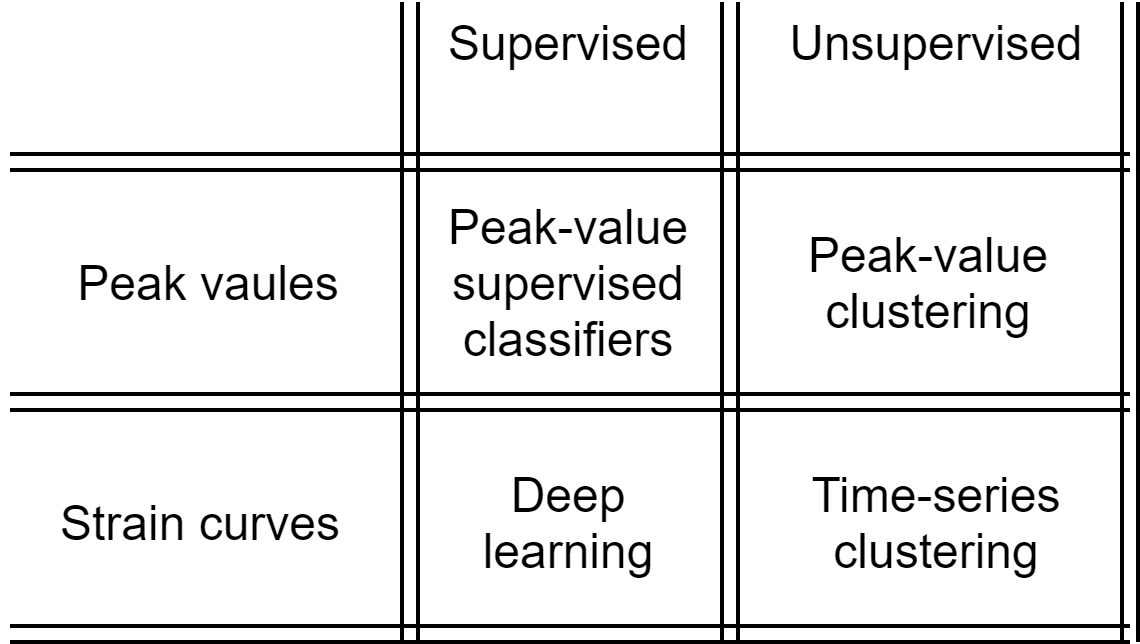
\includegraphics[width=0.5\textwidth]{intro/objectives_diagram.png}
    \caption{This is an illustration of the combinations of strain datasets and machine learning algorithms which will be tested in this work.}
    \label{fig:objectives_diagram}
\end{figure}

The objectives of this work can be summarized in the form of three questions:

\begin{tcolorbox}
    \textbf{Objectives}

    \begin{enumerate}
        \item Can a machine learning model be used to predict one of the three target variables assessed in this work using peak strain values or longitudinal strain curves?
        \item Which type of machine learning is best suited for predicting the aforementioned target variables, supervised or unsupervised learning models?
        \item Which type of input data works best for a machine learning model to predict the target variables, a dataset consisting of longitudinal strain curves or a dataset that consists of peak strain values in combination with \acrshort{ef}?
    \end{enumerate}
\end{tcolorbox}

\section{Structure}

The structure of this work is as follows: Chapter \ref{chap:strain} will explain the theory behind echocardiography, the technology used in ultrasound imaging, and outline the different heart diseases presented. Chapter \ref{chap:ml} describes the theory behind the machine learning models used. Chapter \ref{chap:lit} reviews the most recent work done on the topic. Chapter \ref{chap:data} explores the dataset. Chapter \ref{chap:method} details how every model in this work is configured, trained and evaluated. Chapter \ref{chap:results} presents the results of the individual models tested. A discussion of the results will be made in chapter \ref{chap:discussion} and a conclusion is given in chapter \ref{chap:conclusion}.
\chapter{Method}

This is the section where we detail the specific models used. \bigskip

\section{Models} 

\subsection{Time-series clustering}

\subsection{Peak-value clustering}

\subsection{Recurrent Neural Network}

\subsection{Supervised Peak-value Classifiers}

\section{Description of The Datasets}

Since the different ML models detailed in chapter REFERENCE require different types of input data the, datasets have been divided into two main categories: 
The peak-value datasets and the time-series datasets. \bigskip

\subsection{Time-series Datasets}

\begin{table*}[h]
    \centering
    \ra{1.3}
    \begin{tabular}{ rlr }
        \toprule
        Nr & Input variables   & Shape \\
        \midrule
        1  & Single RLS curves & (3600, 1) \\
        2  & RLS curves        & (200, 18) \\
        3  & GLS curves        & (200, 3)  \\
        4  & Strain curves     & (200, 21) \\
        \bottomrule
    \end{tabular}
    \caption{Time-series datasets. The ''Shape'' parameter is indicates: (Number of objects in the dataset, Number of curves in each individual object). The curve length is not included in the shape parameter because it differs for different curves.}
    \label{tab:ts_dsets}
\end{table*}

Table \ref{tab:ts_dsets} shows the different time-series datasets that will be used. 
All the datasets except \textit{Single RLS curves} will be used to predict the diagnosis of patients, and whether the patient has heart failure.
Recall that the different diagnosises are described in section REFERENCE, and there occurance rate are illustrated in figure \ref{fig:hf_ind_dist}.
\textit{Single RLS curves} will be used to predict the segment indications shown in figure \ref{fig:segm_label_dis} and described in section REFERENCE. 
The point of classifying individual segments of a patients left ventricle is that if a single segment is found to be \textit{not normal}, 
this would also mean that the patient can be considered as \textit{not healthy}.
As mentioned in the description of table \ref{tab:ts_dsets} the ''Shape'' parameter shows how many objects each dataset has, and how many curves are associated to each object. 
Since each ultrasound examination takes ultrasound inspections from three views (four chamber, two chamber, and APLAX chamber), each patient has three views to estimate a GLS curve from. 
Since each GLS curve, also can be divided into six RLS curves, there is a total of 21 strain curves per patient. 
Since each patient has 18 RLS curves, there are $18 \times 200 = 3600$ curves that make up dataset number 1.
Both the RNN, and the TSC model are applied on the datasets listed in table \ref{tab:ts_dsets}, 
\bigskip

\textbf{NOT SURE ABOUT THIS ANYMORE}
however there have been made some significant changes to the multivariate time series to accomodate the DL model.
Even though RNNs are capable of handling objects of different sizes, the curves that make up a single object must be of the same size.
Since the strain curves extracted from different views often are of different lengths, the RNN has been limited to only using the strain curves associated with a single view
when evaluating the diagnosis, or heart failure status of one patient.

\subsection{Peak-value Datasets}

\begin{table*}[h]
    \centering
    \ra{1.3}
    \begin{tabular}{ rlr }
        \toprule
        Nr & Input variables                     & Shape \\
        \midrule                              
        1  & Single peak systolic RLS values     & (3600, 1) \\
        2  & Peak systolic RLS values            & (200, 18) \\
        3  & Peak systolic GLS values            & (200, 3)  \\
        4  & Peak systolic strain values         & (200, 21) \\
        5  & Peak systolic RLS, and EF values    & (200, 19) \\
        6  & Peak systolic GLS, and EF values    & (200, 4)  \\
        7  & Peak systolic strain, and EF values & (200, 22) \\
        \bottomrule
    \end{tabular}
    \caption{Peak-value datasets. The ''Shape'' parameter is indicates: (Number of objects in the dataset, Number of dimensions of each individual object).}
    \label{tab:pv_dsets}
\end{table*}

Table \ref{tab:pv_dsets} shows the different peak-value datasets. 
All the datasets with exception of \textit{Single peak systolic RLS values} will be used to predict the diagnosis of patients, and whether the patient has heart failure. 
\textit{Single peak systolic RLS values} is also the only peak-value dataset that is not suited for clustering, as a minimum of two dimensions is required to cluster a point-value dataset.
The reason that there are more peak-value datasets than there are time-series datasets, is that the peak-value version of three datasets in table \ref{tab:ts_dsets} have been combined 
with EF to determine whether a combination of peak systolic strain and EF can have a higher predictive power than strain alone.

\section{Case Studies}
The results of this paper will be presented in the form of three case studies. 
Each case study will focus on a single target variable, and aims to find which model group performs best at predicting the target variable in question.

Recall that the three target variables that will be considered in this thesis are: Heart failure, patient diagnosis, and the indication of individual left ventricle segments.
As mentioned previously in this chapter there are four main machine learning models that will be tested, but also many variations of these four models.
The variations within the main model categories differ slightly for the different subgroups. 
For the peak-value clustering models the variation between models is what dataset the model is applied on, what linkage is used to define the distance between cluster prototypes, and which number of clusters one chooses to divide the dataset into. 
For the time-series clustering models the variations are choice of dataset, which type of preprocessing is used, what linkage is used and the number of clusters.
For the RNN, the variations are choice of dataset and the type of preprocessing used. 
The main group of peak-value classifiers is a broad group which encompasses ten complex machine learning classifiers. 
No changes will be made to the hyperparameters of the individual models, so the variations in this group will be which particular classifier is used and which dataset the models are applied on. 
In each case study a brief discussion of performance of different model variations within each main category will be made, 
and then the best model variation will be used to compare the performance of the model groups.


\chapter{Discussion}

In the results chapter, the performance results were presented in the order of the different target variables that were explored. 
In the discussion chapter a different approach is taken, and the each model will be discussed individually based on their performance in the case studies.

\section{Time-series Clustering} \label{sec:disc_tsc}

% \textbf{Give a brief summary of how the TSC model was implemented.}
Before dissimilarity was measured between strain curves, curves were preprocessed in one of four ways. 
Curves were either: not preprocessed, scaled between zero and one, normalized between zero and one or z-score normalized.
The TSC model was implemented by using DTW distance between strain curves as a dissimilarity measure to achieve a shape-based TSC model.
All the dissimilarity measures between a specific strain curve of one patient to the same strain curve of every other patient were combined into a dissimilarity matrix.
If the dataset represented patients with more than one strain curve the dissimilarity matrices of each indivial strain curves were added together, such that there was a single dissimilarity matrix that represented the dissimilarity between the patients.
The dissimilarity matrix was then passed to the hierarchical agglomorative clustering algorithm which started out with each patient as an indivial cluster, and merged clusters together based on a specific linkage criteria.
Seven linkage criteria were tested: single, complete, average, ward, centroid, median and weighted.
The clustering model was calculated at the different number of cluster centers between two and nine.
The ARI was estimated for the all the cluster assignments generated, and the different target variables.
For the cluster assignments yielded by a clustering model evaluated at two cluster centers the accuracy, sensitivity, specicity and DOR was also calculated. \bigskip

% \textbf{Mention briefly which placements TSC has in the different case studies.}
The TSC models did not perform best in any of the case studies, but variations of the TSC models generally yielded results with high performance in terms of accuracy, sensitivity and specicity.
In the heart failure case study the best variation of the TSC model achieved the highest sensitivity and DOR, but it was outperformed by the best variation of the PVC model overall.
In the patient diagnosis case study the best variation of the TSC model outperformed the best variation of the PVC model, but they were both outperformed by the best PVSC model.
In the segment indication case study the best variation of the TSC model attains the highest accuracy, specicity and DOR, but is outperformed by the NN because it attains a higher sensitivity score, and thereby attains a more balanced accuracy in the positives and negatives.
% \textbf{Discuss why methods using data from single view performed better.}
As discussed in section REFERENCE, a challenge for all statistical models is the ''curse of dimensionality''. Briefly described, in ML, and data mining the curse of dimensionality refers to the issue of attaining a good balance between the number of dimensions that an object is represented in, and the number of objects used to train and/or evaluate the model. 
In the heart failure and patient diagnoses case studies the TSC models that perform best in terms of DOR, and ARI are the models that use datasets where there are objects are represented by fewer dimensions.
A reason for this could be that for 200 patients, the heart failure diagnoses, and patient diagnoses are most seperable for the TSC models when only one strain curve is used. 
The curve that then gives the easiest separation of patients is then the 2CH GLS curve.
In the heart failure study the TSC models that attain the five best performing models in terms of DOR and ARI only use the GLS curve from the 2CH view, meaning that these methods only use one of 21 possible curves. This can be confirmed from table \ref{tab:tsc_hf_dor_sens_spec_dist} and \ref{tab:tsc_hf_ari}.
In the patient diagnoses study one can see from table \ref{tab:tsc_ind_dor_sens_spec_dist} that the five methods that attain the highest DOR also only use the GLS curve from the 2CH view. 
These two observations support the claim that at a dataset size of 200 objects using fewer strain curves makes it easier for TSC models to separate heart failure diagnoses, and patient diagnoses.
An observation that does not directly support this claim is that in the patient diagnosis case study, the TSC models that attain the four highest ARI use a combination of GLS and RLS curves in the 4CH view, or use the GLS curves from all views.
However, these methods also only use three and seven of 21 curves in total, so this observation does not negate the claim entirely. 
% \textbf{Discuss why methods using data using ''regular'' or ''scaled'' performed better than methods using normalization or z-normalization.}
In all case studies it was found that TSC models that performed best in terms of DOR, and ARI used no preprocessing. 
In some cases models using scaling as a form of preprocessing yielded the same cluster assignments, which could indicate that scaling the curves before measuring dissimilarity does not make much of a difference.
Since TSC models using normalization or z-score normalization as a form of preprocessing were not among the top five methods in terms of DOR, or ARI in any of the case studies the argument could be made that these form of preprocessing are not suited when using DTW as a dissimilarity on left ventrice strain curves.
% \textbf{Talk about the performance of different linkages.}
Of the seven linkages tested, it was the centroid, weighted and ward linkages that went into the TSC models that performed best at predicting heart failure, patient diagnosis and segment indication respectively, in the different case studies. 
However, the single, complete and average linkages also went into the methods that appeared in the top five candidates in terms of DOR, or ARI.
So it is not possible to say certainly that all linkages other than centroid, weighted and ward linkages are not suited for clustering left ventricle strain curves, but one can say with some degree of certainty that the median linkage does not go into any of the TSC models that perform well in any of the three case studies. 
% \textbf{Talk about run-time challenges.}
When calculating the dissimilarity matrix of a set of 200 curves, it took approximately 0.3 seconds using the C-optimized functions of the dtaidistance library.
The time it took to compute the clustering varied between 0.15 and 0.45 seconds depending on what linkage was used. 
The single linkage criteria was found to be the fastest, and the complete linkage was found to be the slowest. 
That the single linkage was the fastest could is to be expected, as it fairly easy to compute. 
However, it was unexpected that the complete linkage was the one that took the longest time to compute as one would expect the more complex linkages such as the ward linkage to take the longest time to compute.
When the size of the dataset was increased to approximately 3600 curves it took 162 seconds to compute the dissimilarity matrix.
This increase in run time is in agreement with the time complexity of the DTW algorithm described in section REFERENCE.
In addition, the time it took to compute the clustering after the dissimilarity matrix was computed also increased to vary between 3 seconds for the single linkage, and 871 seconds for the ward linkage.
So for a bigger dataset the run time of the different linkages were more as expected. 
Although these run-times are attained with a with a regular desktop Lenove G510 laptop, it illustrates possible challenge of how run-time of the calculations of the dissimilarity matrix, and clustering increase quadratically with the size of the dataset.
% \textbf{Improvements that could be done on the existing model}
It was often found that the PVC models that used EF in addition to peak systolic strain values performed better than the PVC models that only used strain values.
It would be interesting to see whether incorporating EF in the TSC model would improve its performance as well.
Since the hierarchical agglomorative clustering algorithm is uses dissimilarity matrix to cluster objects, it should be fairly straight-forward to calculate the dissimilarity matrix between a patients EF values, and add that to the dissimilarity matrices of the indivial curves.
One could also consider the approach taken by CITATION, where they split the strain curves of one heart cycle into systolic, and diastolic strain curves, and pass them to the model separately. 
Although the authors achieved good results with this, they also say that annotating points of every strain curve as systolic or diastolic is very time consuming.

\section{Peak-value Clustering}

% \textbf{Give a brief summary of how the PVC model was implemented.}
The PVC model was implemented in a similar fashion as the TSC model.
The datapoints used to represent patients were passed to an implementation of hierarchical agglomorative clustering in scikit-learn.
The dissimilarity between patients was measured as the Euclidean distance between the dimensions used to represent them.
The scikit-learn implementation did not have all the same clustering linkages available as the scipy implementation used for TSC, so only the following four linkages were tested: single, complete, average and ward.
The evaluation procedure for the PVC model was the same as the procedure used for TSC.
% \textbf{Mention briefly which placements PVC has in the different case studies.}
The best variations of the PVC model had a high performance in the heart failure, and in the patient diagnosis case studies. 
It was chosen as the best model in the heart failure case study, but was closely followed by the TSC, and PVSC models.
In the patient diagnosis case study the best variation of the PVC models attained the highest specicity, and second highest DOR of the three models compared. 
However, it was outperformed by both the TSC, and PVSC models due to its low sensitivity.
% \textbf{Note that the PVC methods that use combination of peak systolic strain values and EF performs significantly better, future work could be to combine EF values with strain curves as well.}
In both case studies PVC models that used datasets that were a combination of peak systolic strain values and EF performed consistently better than the models than only used the strain values. 
This is to some degree expected in the heart failure case study, as EF is parameter that is established in the current medical procedures used to diagnose patients with heart failure.
% \textbf{Talk about the performance of different linkages.}
In the heart failure case study it was the complete linkage which was used in the model that was chosen as the best performer, but the ward, and average linkages were also used in the models that attained the top five DOR and ARI scores.
In the patient diagnosis case study the complete linkages was also used in the model that was chosen as the best performer.
In both case studies where PVC models where tested the models that were chosen as the best performers used the complete linkage, but the average and ward linkages were also used by other model variations that attained the five highest DOR and ARI.
Hence, for PVC models using peak systolic strain values, and EF to identify heart failure among patients, and patient diagnosis the single linkage was not found to be suited.
% \textbf{Talk about run-time challenges.}
Since a scikit learn implementation was used for the PVC model, it was not possible to separate run-time of the dissimilarity calculation and the clustering itself.  
However, Euclidean distance is known to scale linearly with the number of dimensions per object, and number of objects in the dataset.
Since the underlying algorithm used by scikit learn is the same as the one used by scipy it is assumed that it would perform similarily to the TSC model in terms of run time.

\section{Neural Networks}

% \textbf{Give a brief summary of how the NN model was implemented.}
For the NN two types of preprocessing were tested in addition the option of not preprocessing at all, upsampling the curves to the highest sample rate in the dataset and downsampling the curves to the lowest sample rate.
The curves of the dataset were then passed as input to the NN architecture detailed in section REFERENCE together with the relevant target variables.
The NN was trained for five epochs using the backpropagation algorithm and SGD.
To validate the NN models 10-fold cross validation was used, at the end of each fold the TP, TN, FP, and FN of the model were noted. 
After the NN had effectively attempted to predict every object of the dataset all the TP, TN, FP, and FN were summed and this grand total was used to estimate the models accuracy, sensitivity, specicity and DOR.
% \textbf{Mention briefly which placements NN has in the different case studies.}
The NN models performed worst of the four model groups in the heart failure case study, and the patient diagnosis case study.
However, it attained the highest sensitivity in the segment indication case study, and was chosen as the best performing model because its sensitivity and specicity were more balanced than the TSC model.
% \textbf{Talk about performance of NN in different case studies.}
In the patient diagnosis case study close to all of the NN models predicted all the patients to be unhealthy. 
It is evident that a NN with the architecture used in this assignment was not suited to classify patient diagnosies with a skewed dataset of only 170 unhealthy patients and 30 healthy patients.
It is the authors opinion that the reason that the NN models performed so bad at predicting patient diagnosis is an aspect of ''the curse of dimensionality'', and that the network was not able to generalize the characteristics of healthy patients in the study, and therefore minimized loss function by predicting the outcome that was most probable.
From table \ref{tab:dl_hf_raw_results} one can see that the top nine variations of the NN model that performed best in the heart failure case study with regard to DOR, were models that used only the GLS curve from a single view, which supports the claim that 
Since the different NN models differed in architecture depending on how many curves were used to represent one patient, they also varied in the number of trainable parameters they have. 
The NN models which only take a single strain curve as input have 39457 trainable parameters, and the NN models that take 21 curves as input have 80417 trainable parameters.
Even though there is no exact ratio of how big a dataset should be with regard to how many trainable parameters a model has, between 40 and 80 thousand parameters for a dataset of size 200 is likely too many trainable parameters.
On the other hand, the NN model was chosen as the best performing model at predicting segment indication. 
In that case study though the size of the dataset is significantly larger, and each object is represented by a single curve. 
Considering that the architecture of the NN was given, and not developed specifically for this classification problem the performance that the model achieves is significant. 
% \textbf{Possible improvements}
It is the authors opinion that if more time is spent adapting the model to the dataset at hand, even better performances are within reach. 
Especially for the segment indication classification problem where there is so much data, there is potential.
There are alternatives to SGD that could be tested such as batch gradient descent, and the most popular choice mini-batch gradient descent which is a middle road between the two, and is often considered the best alternative REFERENCE.
There is also the GRU cells that are an alternative to the LSTM cells. Like LSTM cells, GRU cells are able capture time-dependent connections. GRU cells are simpler than LSTM cells in composition, and are said to require less training data, to achieve the same accuracies as LSTM cells REFERENCE.
It could also be considered whether it would be beneficial to use some form of dimensionality reduction such as a max pooling layers, which for time series can be considered as a max-filter where only the highest value in a segment of a curve is kept on. 
Dropout layers are also a technique that are used frequently when NN architecture become deep and complex, they introduce the probability that any particular perceptron in the layers preceding the dropout layer can ''drop out'' meaning that they become inactive.
In complex NN architectures it is often found that during training the model becomes overly dependent on certain perceptrons, and specific paths through the network. This leads to the NN not entirely utilizing all the perceptrons at its disposal, and the accuracy suffers. It is found that by adding a probability that any given neuron can drop out during training remedies this effect, and can increase accuracy overall.
% \textbf{Talk about run-time challenges.}
Training, and validating the NN models were one of the more time-consuming computations required.
The time it took to train the network depended on what dataset was used, which makes sense as increasing the number of curves the NN can take as input also increases the number of trainable parameters that need to be trained for each step of the SCG algorithm.
When validating the NN models, a single fold in the 10-fold cross validation took approximately 100 seconds in the heart failure, and patient diagnosis case studies.
The time it took to execute one fold in the segment indication case study took approximately 640 seconds (11 min)
However, these times do not reflect the times it will take to use the NN to evaluate new cases after training, so the same challenge one has with clustering is not as pressing should the aim be to deploy the NN in a real-time clinical setting.

\section{Peak-value Supervised Classifiers} \label{sec:disc_pvsc}

% \textbf{Give a brief summary of how the PVSC model was implemented.}
The different peak-value datasets are passed the different supervised classifiers in the model group. 
The different datasets are detailed in section \ref{sec:datasets}, and the different supervised classifiers tested are detailed in section REFERENCE.
Each combination of dataset and classifiers is validated by a 10-fold cross-validation in the same manner as the NN. 
% \textbf{Mention briefly which placements PVSC has in the different case studies.}
In the heart failure case study the best PVSC model outperformed the best variations of the TSC, and NN models and had a performance that was on par with the PVC, although the best PVC model was ultimately deemed better in the end.
In the patient diagnosis case study the best PVSC model attained the highest accuracy, sensitivity and DOR of the four model groups, and it was deemed the best model group at predict patient diagnosis. 
% \textbf{Mention that DOR distribution of PVSC models were significantly higher centered than the other models groups DOR distribution.}
What should be adressed is the fact that the distribution of the DOR for the different PVSC models, differ from the DOR distributions of the other models in some key ways.
In both the heart failure case study, and the patient diagnosis case study the distribution of DOR for variations of TSC, PVC and NN models are highly concentrated around zero. 
For the PVSC models the lowest DOR attained by a PVSC model in the heart failure study is 1.94, and the lowest DOR attained by a PVSC model in the patient diagnosis case study is 3.68.
In the heart failure case study it is especially evident that the DOR of the different PVSC models is distributed differently than the DOR of the other models.
It can be confirmed from figure \ref{fig:pvmlc_hf_dor_sens_spec_dis} that the distribution of DOR for the PVSC is especially concentrated in the range between four to eight.
The significance of this difference of DOR distribution is two-fold, the first thing to keep in mind is that not very much time was spent optimizing the hyperparameters of the PVSC models as it falls outside the scope of this thesis, and that in contrast to the clustering models the outcome of the PVSC model is probabilistic in the sense that it is highly dependent on the initial conditions of the model before it is trained. 
Since the DOR distribution of PVSC models in the heart failure, and patient diagnosis case studies are distributed higher in general than the TSC and PVC models, and that the PVSC are configured with what can be considered as ''standard hyperparameters'' it is probable that spending time on optimizing the hyperparameters of the PVSC models, and testing different initial conditions could improve the performance of all the PVSC models. 
% \textbf{Talk about run-time challenges.}
The time it took to train and validate the PVSC models varied, and was highly dependent on the dimensions of the dataset and which specific ML model was used. 
The shortest training time encountered was at 201 seconds, and the longest was at 365 seconds.
These were the shortest training times encountered among the four model groups.
Similarily to the NN model the training times of the PVSC models do not hinder their ability to make predictions in real time, and deploy them in a clinical setting.

\chapter{Conclusion}

The main objective of this thesis, as stated in section \ref{sec:objective} have been explore whether a ML model using longitudinal strain values as input can identify whether a patient has heart failure, if a patient has a heart disease and if an individual segment in a patients left ventricle is acting abnormally. The main objective is divided into two sub-objectives that decided the direction and scope of the thesis: Which type of ML model will perform best, a supervised or unsupervised learning model, and what type of longitudinal strain data will yield the best performance for the ML models, longitudinal strain curves or peak systolic strain values in combination with EF. \bigskip

A dataset of 200 patients was used to fulfill these objectives. The models that used combinations of GLS, and RLS curves from different views were a TSC model and an ANN, which were tested to classify heart failure among patients, patient diagnosis and whether individual left ventricle segments were acting abnormally. In addition to varying the dataset used with these models different forms of preprocessing was tested for both models, and different linkages were tested for the TSC model. The models that used peak systolic strain values were a PVC model, and a 11 different PVSC, they were only applied to identify heart failure among patients, and patient diagnosis. To assess the performance of the supervised models accuracy, sensitivity, specificity and DOR were used as evaluation metrics. To evaluate the unsupervised models the same metrics were used as for the supervised models, in addition to using the ARI to determine whether clustering models evaluated at a number of cluster centers greater than two could provide better performance than models evaluated at two cluster centers. When making a choice as to which model variation performed best within their respective model groups, and which model performed best overall the models were sorted in descending order of the DOR score they attained, the models which attained the highest DOR and accuracy while at the same time maintaining a balanced relationship of sensitivity and specificity were then chosen as the best performing models. For the clustering models, an additional evaluation was done with respect to ARI. If there were clustering models evaluated at a number of cluster centers greater than two that attained an ARI greater than the best performing two-cluster-center model, an attempt was made to visualize the result. Further, it was evaluated whether combining the clusters of the model with more than two centers could yield a better performance than the two-cluster-center model. \bigskip

The overall consensus from the results are that it is possible to implement an ML model that uses longitudinal strain as input, and that can predict one of the three target varables. However, there was not a single model that performed best at predicting all the target variables. The model that performed best at identifying heart failure among patients was a variation of the PVC model which used a combination of peak systolic GLS values and EF as input data, used the complete linkage and was evaluated at two cluster centers. This method attained an accuracy of 0.76, sensitivity of 0.81, specificity of 0.72 and DOR of 10.85. The model that performed best at predicting patient diagnosis was one of the PVSC models that used the KNN classifier trained on a combination of peak systolic GLS, and RLS values. It attained an accuracy of 0.93, a sensitivity of 0.95, a specificity of 0.82 and a DOR of 84.53.
In the segment indication case study, the ANN that downsampled all the individual RLS curves to the lowest sample rate of all the curves was chosen as the best model. That model attained an accuracy of 0.74, sensitivity of 0.74, specificity of 0.75 and DOR of 8.38. \bigskip

It was found that PVC, and PVSC models that used a combination of peak strain values and EF generally performed better at predicting heart failure than variations that used peak strain values alone. The ANN was not able to generalize the features of healthy patients in the patient diagnosis case study at all, and did not perform particularily well in the heart failure case study either. It is the authors opinion that this is because the architecture of the ANN is to complex to be trained solely on a dataset of 200 patients. This conclusion was drawn based on the fact that the ANN had between 40 and 80 thousand trainable depending on how many curves were used as input. This statement is also supported by the fact that the ANN performed significantly better, when applied to classify single curves on a dataset of size 3600 curves.

\section{Future Work}

It is the authors opinion that there are two continuations of this work that show good promise. Since the scope of this thesis has been quite wide there has not been enough time to do a deep dive into any of the specific models, so both of the suggestions are deep dives into specific models since a broad comparison has already been made.

\subsection*{Development of an Artificial Neural Network for Segment Indication}

Given that the ANN performed so well at identifying the binary segment indication, it is probable that by spending more time adapting the architecture to the segment indication dataset one could achieve performances that are better than the ones attained in this piece of work. One could start with the architecture used in this assignment, and attempt to reduce the complexity of the architecture by adding pooling layers, or dropout layers. In addition, it should be tested whether using GRU cells could could improve the accuracy of the ANN as they are known to require less data than LSTM cells to generalize the difference between different segment labels. If concentrating mainly on an ANN solution one could also test if the resulting model is capable of dealing with segment indication when multiple classes are used. 

\subsection*{Development of Peak-value Supervised classifiers}

As mentioned in section \ref{sec:disc_pvsc}, although the PVSC did not perform best at identifying heart failure in patients, the distribution of the DOR for the PVSC models was shifted significantly higher, and centered higher than the DOR distribution of the TSC, PVC and ANN models. Since there was not time to optimize the hyperparameters of the individual classifiers in the PVSC group, this shift in distribution indicates that there is some lost potential as to what performance these models could attain. Therefore, it is probable that by spending more time on adapting the individual classifiers to the heart failure, and patient diagnosis datasets one could produce models that yield higher scores in all evaluation metrics.

% \include{appendix/time_warping_figures}
% \include{appendix/code}

\printbibliography

\end{document}
